\documentclass[border=0]{standalone}
% \documentclass[a4paper]{article}
% \usepackage[left=-2mm,top=2mm,right=0mm,bottom=0mm]{geometry}
\usepackage{tikz}
\begin{document}
% \thispagestyle{empty}

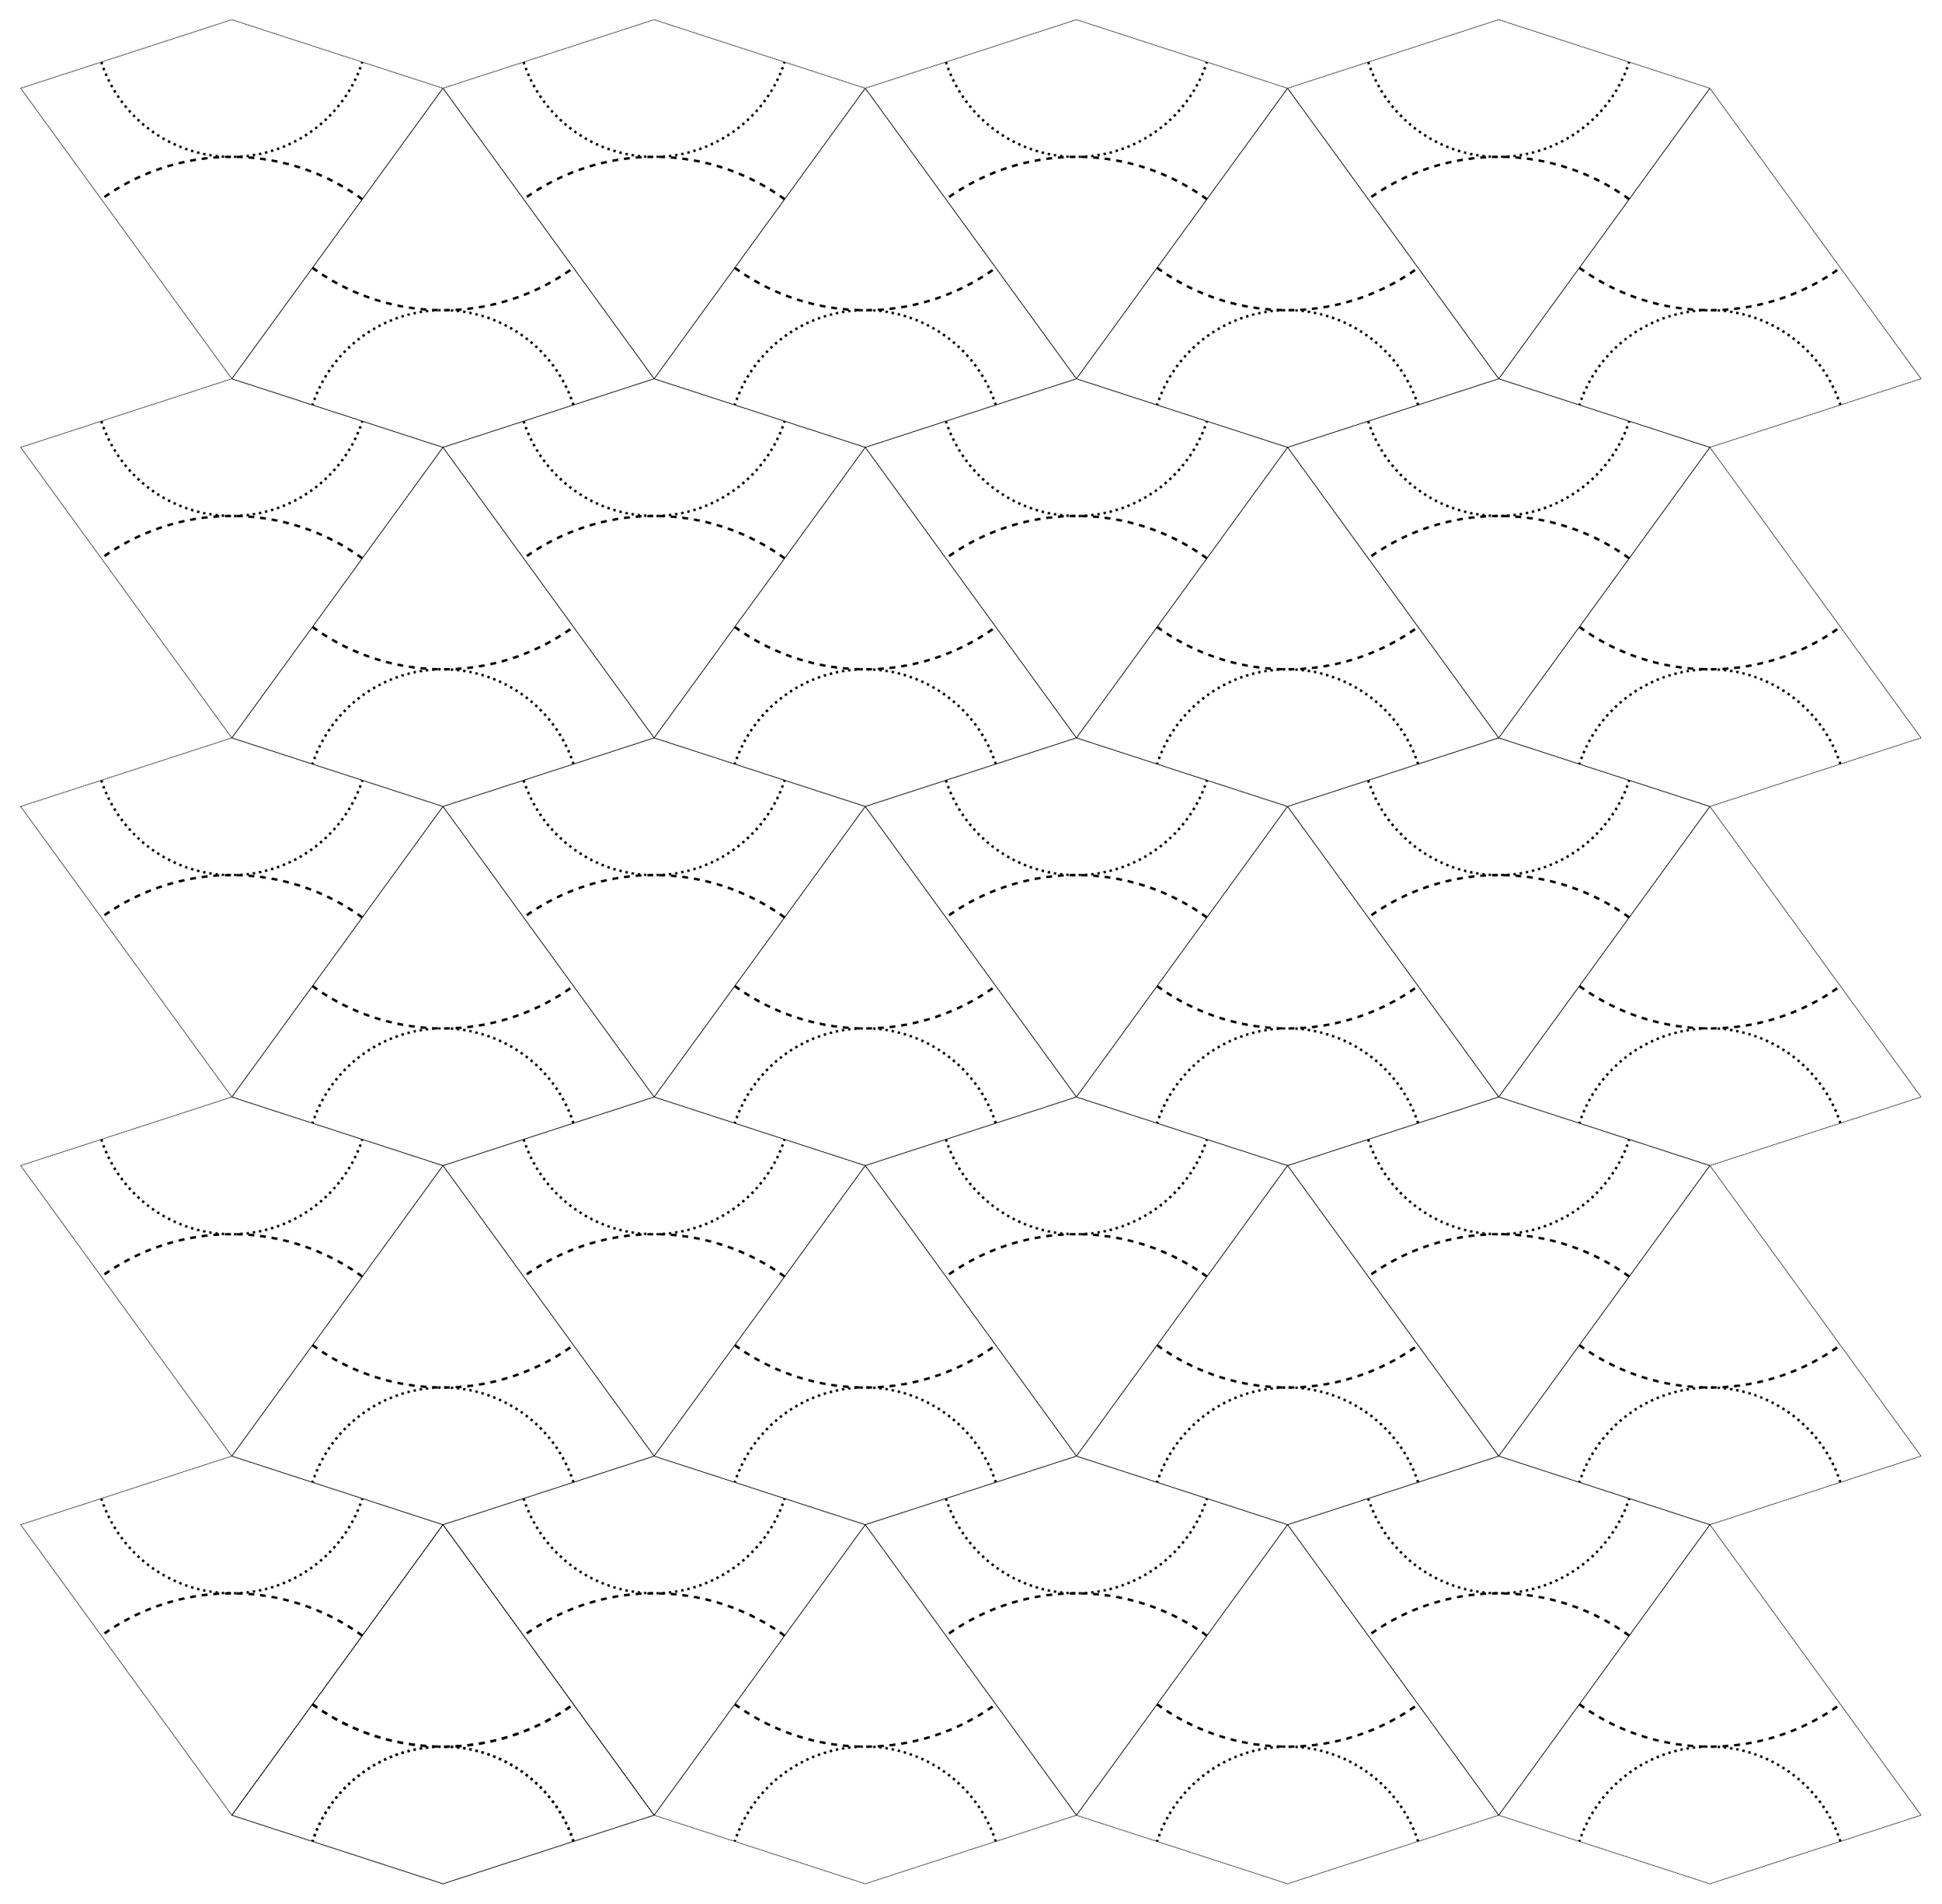
\begin{tikzpicture}
    \pgfmathsetmacro{\p}{(1+sqrt(5))/2}
    \pgfmathsetmacro{\w}{4}
    \tikzset{
        kite/.pic={
            \draw[very thin] (0,0)--++(0:\w*\p) --++ (108:\w) --++ (144:\w)--cycle;
            \draw[dashed, very thick] (0:\w) arc (0:72:\w);
            \draw[dotted, very thick] (72:\p*\w)++(-36:{\w/(1+\p)}) arc (144:288:\w/\p);
        }
    }
    \draw ({\p*\w*cos(54)},{\p*\w*sin(54)}) pic [rotate=-126] {kite};
    \foreach \x in {0,1,2,...,3}{
        \foreach \y in {0,1,2,...,4}{
            \draw ({2*\p*\w*cos(54)*\x},{(\p*sin(54)+sin(18))*\w*\y}) pic [rotate=54] {kite};
            \draw ({\p*\w*cos(54)+2*\p*\w*cos(54)*\x},{\p*\w*sin(54)+(\p*sin(54)+sin(18))*\w*\y}) pic [rotate=-126] {kite};
        }
    };
\end{tikzpicture}
\end{document}